% !TeX program = xelatex
\documentclass[a4paper,10pt]{article}

% ============================================================================
% កញ្ចប់បណ្ណាល័យ (Packages) – តាមលំនាំ NGS Preah Krasang (ls_plan.tex)
% ============================================================================
\usepackage[a4paper, left=0.95cm, right=0.95cm, top=0.85cm, bottom=0.92cm, footskip=0.52cm]{geometry}
\usepackage{amsmath}
\usepackage{unicode-math}
\usepackage{fontspec}
\usepackage{array, longtable, multirow, colortbl}
\usepackage[table]{xcolor}
\usepackage{enumitem}
\usepackage{pifont}
\usepackage{fancyhdr}
\usepackage{tikz}
\usetikzlibrary{calc, arrows.meta, angles, quotes, decorations.markings, babel}

% LaTeX 2025 + longtable v4.24 compatibility guard
\makeatletter
\let\@expl@@@mark@update@singlecol@structures@@\relax
\makeatother

% ============================================================================
% ការកំណត់ពុម្ពអក្សរ (Fonts Configuration) – តាមលំនាំស្ដង់ដារ ១០០%
% ============================================================================
% Cross-platform font path resolver (Windows local + Linux/Cloud repo fonts/)
\providecommand{\NGSFindFonts}{%
  \IfFileExists{C:/Windows/Fonts/cambria.ttc}{%
    \def\NGSSysPath{C:/Windows/Fonts/}%
    \def\NGSUserPath{C:/Users/KIT/AppData/Local/Microsoft/Windows/Fonts/}%
  }{%
    \IfFileExists{./fonts/KhmerOSsiemreap.ttf}{\def\NGSSysPath{./fonts/}\def\NGSUserPath{./fonts/}}{%
    \IfFileExists{../fonts/KhmerOSsiemreap.ttf}{\def\NGSSysPath{../fonts/}\def\NGSUserPath{../fonts/}}{%
    \IfFileExists{../../fonts/KhmerOSsiemreap.ttf}{\def\NGSSysPath{../../fonts/}\def\NGSUserPath{../../fonts/}}{%
    \IfFileExists{../../../fonts/KhmerOSsiemreap.ttf}{\def\NGSSysPath{../../../fonts/}\def\NGSUserPath{../../../fonts/}}{%
    \IfFileExists{../../../../fonts/KhmerOSsiemreap.ttf}{\def\NGSSysPath{../../../../fonts/}\def\NGSUserPath{../../../../fonts/}}{%
    \IfFileExists{../../../../../fonts/KhmerOSsiemreap.ttf}{\def\NGSSysPath{../../../../../fonts/}\def\NGSUserPath{../../../../../fonts/}}{%
    \IfFileExists{../../../../../../fonts/KhmerOSsiemreap.ttf}{\def\NGSSysPath{../../../../../../fonts/}\def\NGSUserPath{../../../../../../fonts/}}{%
      \def\NGSSysPath{../../../../../../../fonts/}\def\NGSUserPath{../../../../../../../fonts/}%
    }}}}}}}%
  }%
}
\NGSFindFonts

\setmathfont[
  Path={\NGSSysPath},
  FontIndex=1,
  Scale=1.02
]{cambria.ttc}

\defaultfontfeatures{Ligatures=TeX}

\setmainfont[
  Path={\NGSUserPath},
  Extension=.ttf,
  Script=Khmer,
  BoldFont={KhmerOSsiemreap},
  BoldFeatures={FakeBold=1.8},
  ItalicFont={KhmerOSsiemreap},
  ItalicFeatures={FakeSlant=0.25},
  BoldItalicFont={KhmerOSsiemreap},
  BoldItalicFeatures={FakeBold=1.8, FakeSlant=0.25}
]{KhmerOSsiemreap}

\newfontfamily\muol[
  Path={\NGSUserPath},
  Extension=.ttf,
  Script=Khmer
]{KhmerOSmuollight}

\newfontfamily\TimesEn[
  Path={\NGSSysPath},
  Extension=.ttf,
  Scale=1.00,
  BoldFont={timesbd},
  ItalicFont={timesi},
  BoldItalicFont={timesbi}
]{times}

\newfontfamily\NagaBold[
  Path={\NGSUserPath},
  Extension=.ttf
]{AKbalthom Naga Bold}

\newfontfamily\CalibriFont[
  Path={\NGSSysPath},
  Extension=.ttf
]{calibri}

\newfontfamily\Tacteing[
  Path={\NGSUserPath}
]{TACTENG.TTF}

\newfontfamily\CourierBullet[
  Path={\NGSSysPath},
  Extension=.ttf
]{cour}
\newcommand{\wcirc}{{\CourierBullet\fontsize{9.5pt}{11pt}\selectfont o}}

% ក្បួនកាត់ពាក្យខ្មែរ (Khmer word wrapping)
\XeTeXlinebreaklocale "km"
\XeTeXlinebreakskip = 0pt plus 1pt minus 0.1pt

% ============================================================================
% ការកំណត់ពណ៌ និងទម្រង់ទំព័រ (Colors & Page Style)
% ============================================================================
\definecolor{stepgray}{HTML}{D9D9D9}
\definecolor{headgray}{HTML}{F2F2F2}
\definecolor{boxgray}{HTML}{D9D9D9}
\definecolor{darkred}{HTML}{C00000}
\definecolor{red5e}{HTML}{FF0000}

\pagestyle{fancy}
\fancyhf{}
\renewcommand{\headrulewidth}{0pt}
\fancyfoot[R]{\CalibriFont\fontsize{11pt}{13pt}\selectfont\thepage}

\setlength{\parindent}{0pt}
\setlength{\parskip}{0pt}
\setlength{\tabcolsep}{3.8pt}

\newcolumntype{L}[1]{>{\raggedright\arraybackslash}p{#1}}

% ============================================================================
% ម៉ាក្រូជំនួយ (Helper Macros)
% ============================================================================
\newcommand{\en}[1]{{\TimesEn #1}}
\newcommand{\enbf}[1]{{\TimesEn\textbf{#1}}}
\newcommand{\unit}[1]{\,\text{\en{#1}}}
\newcommand{\fiveE}[1]{{\NagaBold\fontsize{9.5pt}{13pt}\selectfont\textcolor{red5e}{#1}}}
\newcommand{\timenote}[1]{\textcolor{darkred}{\textit{#1}}}
\newcommand{\redsub}[1]{\textcolor{darkred}{#1}}
\newcommand{\graybox}[1]{\colorbox{boxgray}{\strut\hspace{2pt}#1\hspace{2pt}}}
\newcommand{\ditem}{\tikz[baseline=-0.5ex]\fill (0,0.42ex) -- (0.42ex,0) -- (0,-0.42ex) -- (-0.42ex,0) -- cycle;\hspace{0.3em}}
\newcommand{\cnum}[1]{{\fontsize{10.5pt}{12pt}\selectfont\ding{\numexpr181+#1\relax}}\hspace{0.2em}}
\newcommand{\cfig}[1]{\par\vspace{4pt}{\centering #1\par}\vspace{4pt}}
\newcommand{\stepheader}[1]{\multicolumn{3}{|c|}{\cellcolor{stepgray}\muol #1} \\* \noalign{\hrule height 0.4pt}}
\newcommand{\tri}[1]{\ensuremath{\triangle #1}}
\newcommand{\ang}[1]{\ensuremath{\angle #1}}
\newcommand{\cg}{\ensuremath{\cong}}
\newcommand{\ncg}{\ensuremath{\not\cong}}

% រចនាប័ទ្មគូសសម្គាល់ជ្រុងស្មើគ្នា (Tick mark styles - bold B&W print safe)
\tikzset{
  tk1/.style={postaction={decorate},decoration={markings,mark=at position 0.50 with {\draw[black, line width=0.85pt](0,-0.095)--(0,0.095);}}},
  tk2/.style={postaction={decorate},decoration={markings,
    mark=at position 0.45 with {\draw[black, line width=0.85pt](0,-0.095)--(0,0.095);},
    mark=at position 0.55 with {\draw[black, line width=0.85pt](0,-0.095)--(0,0.095);}}},
  tk3/.style={postaction={decorate},decoration={markings,
    mark=at position 0.42 with {\draw[black, line width=0.85pt](0,-0.095)--(0,0.095);},
    mark=at position 0.50 with {\draw[black, line width=0.85pt](0,-0.095)--(0,0.095);},
    mark=at position 0.58 with {\draw[black, line width=0.85pt](0,-0.095)--(0,0.095);}}},
  tkslash/.style={postaction={decorate},decoration={markings,mark=at position 0.50 with {\draw[black, line width=0.85pt](-0.065,-0.075)--(0.065,0.075);}}},
  hypArrow/.style={black, densely dashed, line width=0.8pt, -{Stealth[length=3.5pt]}}
}

% ម៉ាក្រូគូសប្រអប់មុំកែង 90° ត្រង់ #3 ក្នុងមុំ #2-#3-#4
\newcommand{\rightbox}[4][0.19]{%
  \draw[black, line width=0.8pt]
    ($(#3)!#1!(#2)$) -- ($($(#3)!#1!(#2)$)+($(#3)!#1!(#4)$)-(#3)$) -- ($(#3)!#1!(#4)$);
}

% ក្បាច់ក្រោមបាវចនា (Tacteing Font - Keyboard '3')
\newcommand{\khmflourish}{{\Tacteing\fontsize{36pt}{14pt}\selectfont\raisebox{-5pt}{3}}}

% ============================================================================
% ម៉ាក្រូគូសរូបធរណីមាត្រ (Monochrome B&W TikZ Figures, 100% Black Text)
% ============================================================================

% ១. កំណែកិច្ចការផ្ទះមេរៀនមុន (លំហាត់ #1, #3, #5 ទំ.១៦៤)
\newcommand{\figHWoldISO}{%
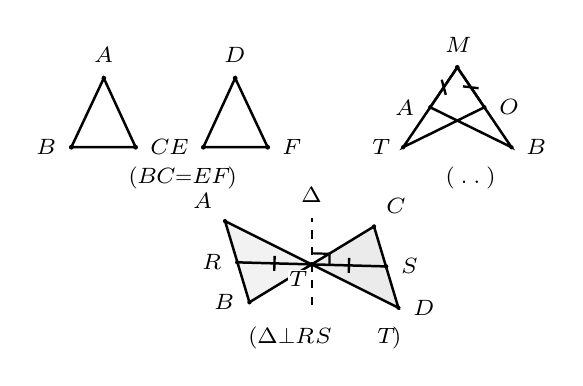
\begin{tikzpicture}[scale=0.86, every node/.style={font=\footnotesize, text=black}]
  % ទី១៖ △ABC ≅ △DEF (ជួរលើឆ្វេង)
  \begin{scope}[shift={(-3.55,2.05)}]
    \coordinate (B) at (0,0);
    \coordinate (C) at (0.95,0);
    \coordinate (A) at (0.48,1.02);
    \draw[black, line width=0.9pt] (A) -- (B) -- (C) -- cycle;
    \fill[black] (A) circle (1.0pt) node[above=2pt] {$A$};
    \fill[black] (B) circle (1.0pt) node[left=2pt] {$B$};
    \fill[black] (C) circle (1.0pt) node[right=2pt] {$C$};
    \coordinate (E) at (1.95,0);
    \coordinate (F) at (2.90,0);
    \coordinate (D) at (2.42,1.02);
    \draw[black, line width=0.9pt] (D) -- (E) -- (F) -- cycle;
    \fill[black] (D) circle (1.0pt) node[above=2pt] {$D$};
    \fill[black] (E) circle (1.0pt) node[left=2pt] {$E$};
    \fill[black] (F) circle (1.0pt) node[right=2pt] {$F$};
    \node at (1.45,-0.45) {ទី១ ($BC{=}EF$)};
  \end{scope}
  % ទី៣៖ MT=MB, MA=MO (ជួរលើស្ដាំ)
  \begin{scope}[shift={(2.15,2.05)}]
    \coordinate (M) at (0,1.18);
    \coordinate (T) at (-0.80,0);
    \coordinate (B) at (0.80,0);
    \coordinate (A) at ($(M)!0.50!(T)$);
    \coordinate (O) at ($(M)!0.50!(B)$);
    \draw[black, line width=0.9pt] (M) -- (T) -- (O) (M) -- (B) -- (A);
    \draw[black, line width=0.85pt, tkslash] (M) -- (A);
    \draw[black, line width=0.85pt, tkslash] (M) -- (O);
    \fill[black] (M) circle (1.0pt) node[above=2pt] {$M$};
    \fill[black] (A) circle (0.9pt) node[left=2pt] {$A$};
    \fill[black] (O) circle (0.9pt) node[right=2pt] {$O$};
    \fill[black] (T) circle (0.9pt) node[left=2pt] {$T$};
    \fill[black] (B) circle (0.9pt) node[right=2pt] {$B$};
    \node at (0,-0.45) {ទី៣ (ជ.ម.ជ)};
  \end{scope}
  % ទី៥៖ AB∥CD, TR=TS, Δ⊥RS ត្រង់ T (ជួរក្រោមកណ្ដាល)
  \begin{scope}[shift={(0,0.32)}]
    \coordinate (T) at (0,0);
    \coordinate (A) at (-1.28,0.64);
    \coordinate (B) at (-0.92,-0.56);
    \coordinate (C) at (0.92,0.56);
    \coordinate (D) at (1.28,-0.64);
    \coordinate (R) at (-1.10,0.03);
    \coordinate (S) at (1.10,-0.03);
    \fill[gray!10] (A) -- (B) -- (T) -- cycle;
    \fill[gray!16] (C) -- (D) -- (T) -- cycle;
    \draw[black, line width=0.9pt] (A) -- (B) -- (C) -- (D) -- (A);
    \draw[black, line width=0.9pt, tk1] (R) -- (T);
    \draw[black, line width=0.9pt, tk1] (T) -- (S);
    \coordinate (Dbot) at (0,-0.60);
    \coordinate (Dtop) at (0,0.68);
    \draw[black, line width=0.85pt, dashed] (Dbot) -- (Dtop) node[above=2pt] {$\Delta$};
    \rightbox[0.24]{Dtop}{T}{S}
    \fill[black] (A) circle (0.9pt) node[above left=1pt] {$A$};
    \fill[black] (B) circle (0.9pt) node[left=2pt] {$B$};
    \fill[black] (C) circle (0.9pt) node[above right=1pt] {$C$};
    \fill[black] (D) circle (0.9pt) node[right=2pt] {$D$};
    \fill[black] (T) circle (1.0pt) node[below left=2pt, fill=white, inner sep=0.4pt] {$T$};
    \fill[black] (R) circle (0.9pt) node[left=2pt] {$R$};
    \fill[black] (S) circle (0.9pt) node[right=2pt] {$S$};
    \node at (0,-1.08) {ទី៥ ($\Delta{\perp}RS$ ត្រង់ $T$)};
  \end{scope}
\end{tikzpicture}}

% ២. រំលឹកមេរៀនទាក់ទង៖ វាក្យសព្ទត្រីកោណសមបាទ និងបន្ទាត់ពិសេសទាំង ៤
\newcommand{\figPrereqISO}{%
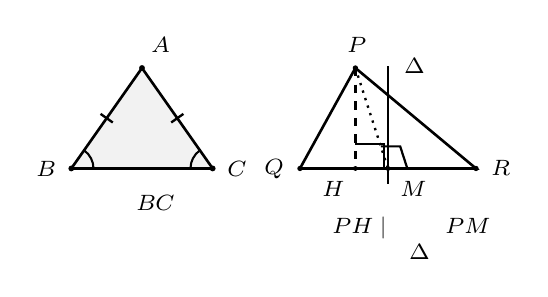
\begin{tikzpicture}[scale=0.88, every node/.style={font=\footnotesize, text=black}]
  % ឆ្វេង៖ ត្រីកោណសមបាទ ABC
  \begin{scope}[shift={(-2.10,0)}]
    \coordinate (A) at (0,1.45);
    \coordinate (B) at (-1.02,0);
    \coordinate (C) at (1.02,0);
    \fill[gray!10] (A) -- (B) -- (C) -- cycle;
    \draw[black, line width=0.95pt, tk1] (A) -- (B);
    \draw[black, line width=0.95pt, tk1] (A) -- (C);
    \draw[black, line width=0.95pt] (B) -- (C);
    \draw[black, line width=0.75pt] ($(B)+(0:0.32)$) arc (0:54:0.32);
    \draw[black, line width=0.75pt] ($(C)+(180:0.32)$) arc (180:126:0.32);
    \fill[black] (A) circle (1.2pt) node[above=2pt] {កំពូល $A$};
    \fill[black] (B) circle (1.2pt) node[left=2pt] {$B$};
    \fill[black] (C) circle (1.2pt) node[right=2pt] {$C$};
    \node[below=4pt] at (0,-0.08) {បាទ $BC$};
  \end{scope}
  % ស្ដាំ៖ បន្ទាត់ពិសេស ៣ កាត់កំពូល vs មេដ្យាទ័រមិនបាច់កាត់កំពូល
  \begin{scope}[shift={(1.40,0)}]
    \coordinate (P) at (-0.42,1.45);
    \coordinate (Q) at (-1.22,0);
    \coordinate (R) at (1.32,0);
    \coordinate (M) at (0.05,0);
    \coordinate (H) at (-0.42,0);
    \draw[black, line width=0.95pt] (P) -- (Q) -- (R) -- cycle;
    \draw[black, line width=0.85pt, dashed] (P) -- (H);
    \rightbox[0.24]{P}{H}{R}
    \draw[black, line width=0.85pt, dotted] (P) -- (M);
    \draw[black, line width=0.95pt] (0.05,-0.22) -- (0.05,1.48) node[right=2pt] {$\Delta$};
    \rightbox[0.22]{P}{M}{R}
    \fill[black] (P) circle (1.1pt) node[above=2pt] {$P$};
    \fill[black] (Q) circle (1.1pt) node[left=2pt] {$Q$};
    \fill[black] (R) circle (1.1pt) node[right=2pt] {$R$};
    \fill[black] (H) circle (1.0pt) node[below left=1pt] {$H$};
    \fill[black] (M) circle (1.0pt) node[below right=1pt] {$M$};
    \node[below=4pt, align=center] at (0.05,-0.40) {កម្ពស់ $PH$ $\vert$ មេដ្យាន $PM$\\មេដ្យាទ័រ $\Delta$};
  \end{scope}
\end{tikzpicture}}

% ៣. E1 Engage: ហោជាងសាលាឆទាន (ខ្សែប្រយោលកែង) និងប៉មទឹកផ្ទះ ៣ ខ្នង
\newcommand{\figEngageISO}{%
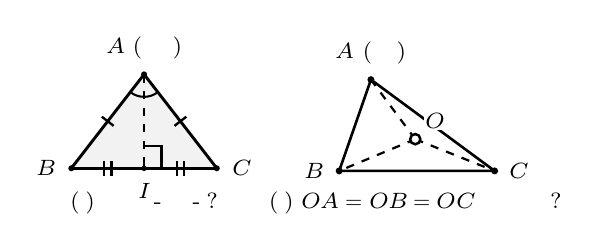
\begin{tikzpicture}[scale=0.84, every node/.style={font=\footnotesize, text=black}]
  % (១) ហោជាងសាលាឆទាន
  \begin{scope}[shift={(-2.20,0)}]
    \coordinate (A) at (0,1.42);
    \coordinate (B) at (-1.10,0);
    \coordinate (C) at (1.10,0);
    \coordinate (I) at (0,0);
    \fill[gray!10] (A) -- (B) -- (C) -- cycle;
    \draw[black, line width=1.05pt, tk1] (A) -- (B);
    \draw[black, line width=1.05pt, tk1] (A) -- (C);
    \draw[black, line width=1.0pt, tk2] (B) -- (I);
    \draw[black, line width=1.0pt, tk2] (I) -- (C);
    \draw[black, line width=0.9pt, dashed] (A) -- (I);
    \rightbox[0.24]{A}{I}{C}
    \draw[black, line width=0.75pt] ($(A)+(-128:0.34)$) arc (-128:-90:0.34);
    \draw[black, line width=0.75pt] ($(A)+(-90:0.34)$) arc (-90:-52:0.34);
    \fill[black] (A) circle (1.3pt) node[above=2pt] {$A$ (កំពូល)};
    \fill[black] (B) circle (1.3pt) node[left=2pt] {$B$};
    \fill[black] (C) circle (1.3pt) node[right=2pt] {$C$};
    \fill[black] (I) circle (1.2pt) node[below=2pt] {$I$};
    \node at (0,-0.52) {(១) ហោជាង៖ ៤-ក្នុង-១?};
  \end{scope}
  % (២) ផ្ទះ ៣ ខ្នង និងប៉មទឹក O
  \begin{scope}[shift={(1.85,0)}]
    \coordinate (A) at (-0.62,1.34);
    \coordinate (B) at (-1.10,-0.04);
    \coordinate (C) at (1.25,-0.04);
    \coordinate (O) at (0.05,0.44);
    \draw[black, line width=0.95pt] (A) -- (B) -- (C) -- cycle;
    \draw[black, line width=0.8pt, dashed] (O) -- (A);
    \draw[black, line width=0.8pt, dashed] (O) -- (B);
    \draw[black, line width=0.8pt, dashed] (O) -- (C);
    \fill[black] (A) circle (1.5pt) node[above=2pt] {$A$ (ផ្ទះ)};
    \fill[black] (B) circle (1.5pt) node[left=2pt] {$B$};
    \fill[black] (C) circle (1.5pt) node[right=2pt] {$C$};
    \draw[black, fill=white, line width=0.9pt] (O) circle (2.2pt);
    \node[above right=3pt, fill=white, inner sep=0.5pt] at (O) {$O$};
    \node at (0.05,-0.52) {(២) $OA=OB=OC$៖ ក្នុងឬក្រៅ?};
  \end{scope}
\end{tikzpicture}}

% ៤. E2 Act 1: បត់ក្រដាស ១:១ (△ABC សមបាទទ្រេត 12° vs △PQR កំពូលខុស Q)
\newcommand{\figExploreOneISO}{%
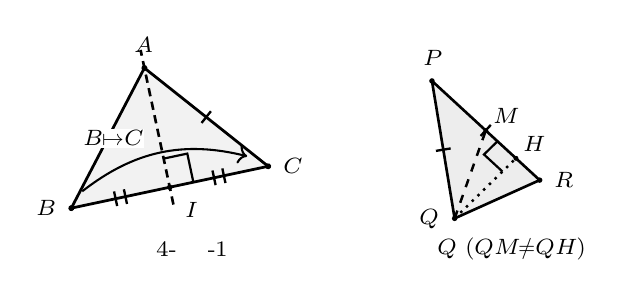
\begin{tikzpicture}[scale=0.90, every node/.style={font=\footnotesize, text=black}]
  % ឆ្វេង៖ △ABC សមបាទទ្រេត 12° (BC=6.0, AB=AC=5.0, AI=4.0)
  \begin{scope}[shift={(-2.15,0.12)}, rotate=12]
    \coordinate (B) at (-1.42,0);
    \coordinate (C) at (1.42,0);
    \coordinate (I) at (0,0);
    \coordinate (A) at (0,1.72);
    \fill[gray!10] (A) -- (B) -- (C) -- cycle;
    \draw[black, line width=1.0pt, tk1] (A) -- (B);
    \draw[black, line width=1.0pt, tk1] (A) -- (C);
    \draw[black, line width=1.0pt, tk2] (B) -- (I);
    \draw[black, line width=1.0pt, tk2] (I) -- (C);
    \draw[black, line width=0.95pt, densely dashed] (0,-0.25) -- (0,1.98);
    \rightbox[0.24]{A}{I}{C}
    \draw[black, line width=0.75pt, ->, bend left=26] (-1.22,0.20) to (1.16,0.20);
    \node[fill=white, inner sep=0.5pt] at (-0.82,0.88) {បត់ $B{\mapsto}C$};
    \fill[black] (A) circle (1.2pt) node[above=2pt] {$A$};
    \fill[black] (B) circle (1.2pt) node[left=2pt] {$B$};
    \fill[black] (C) circle (1.2pt) node[right=2pt] {$C$};
    \fill[black] (I) circle (1.1pt) node[below right=2pt] {$I$};
  \end{scope}
  \node at (-2.15,-0.75) {សមបាទ៖ $4$-ក្នុង-$1$};
  % ស្ដាំ៖ រូបបង្គាប់កំពូលខុស △PQR (PQ=PR=4.5, QR=3.0; គូសពី Q)
  \begin{scope}[shift={(1.55,0)}]
    \coordinate (P) at (0,1.62);
    \coordinate (R) at (1.52,0.22);
    \coordinate (Q) at (0.32,-0.32);
    \coordinate (M) at ($(P)!0.50!(R)$);
    \coordinate (H) at ($(P)!0.78!(R)$);
    \fill[gray!14] (P) -- (Q) -- (R) -- cycle;
    \draw[black, line width=0.95pt, tk1] (P) -- (Q);
    \draw[black, line width=0.95pt, tk1] (P) -- (R);
    \draw[black, line width=0.95pt] (Q) -- (R);
    \draw[black, line width=0.9pt, dashed] (Q) -- (M);
    \draw[black, line width=0.9pt, dotted] (Q) -- (H);
    \rightbox[0.22]{Q}{H}{P}
    \fill[black] (P) circle (1.1pt) node[above=2pt] {$P$};
    \fill[black] (Q) circle (1.1pt) node[left=2pt] {$Q$};
    \fill[black] (R) circle (1.1pt) node[right=2pt] {$R$};
    \fill[black] (M) circle (1.0pt) node[above right=2pt, fill=white, inner sep=0.4pt] {$M$};
    \fill[black] (H) circle (1.0pt) node[above right=2pt, fill=white, inner sep=0.4pt] {$H$};
    \node at (0.72,-0.75) {កំពូលខុស $Q$ ($QM{\neq}QH$)};
  \end{scope}
\end{tikzpicture}}

% ៥. E2 Act 2 Dual POE: Panel A (មុំស្រួច O ក្នុង) vs Panel B (មុំទាល 115° O' ក្រៅ)
\newcommand{\figExploreTwoISO}{%
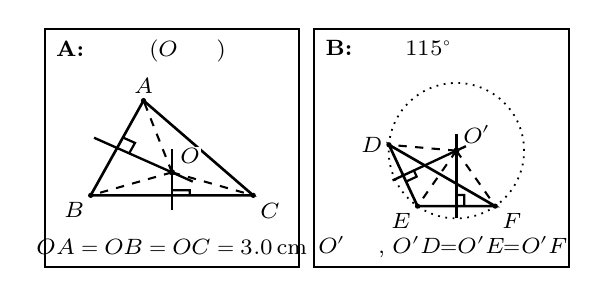
\begin{tikzpicture}[scale=0.86, every node/.style={font=\footnotesize, text=black}]
  % Panel A: Acute Scalene ABC (O inside)
  \begin{scope}[shift={(0,0)}]
    \draw[black, line width=0.8pt] (-1.88,-1.18) rectangle (1.88,2.34);
    \node[anchor=north west, inner sep=3pt] at (-1.84,2.30) {\textbf{A:} មុំស្រួច ($O$ ក្នុង)};
    \coordinate (O) at (0,0.22);
    \coordinate (A) at (-0.42,1.28);
    \coordinate (B) at (-1.20,-0.12);
    \coordinate (C) at (1.20,-0.12);
    \coordinate (L) at ($(A)!0.5!(B)$);
    \coordinate (M) at ($(B)!0.5!(C)$);
    \draw[black, line width=0.95pt] (A) -- (B) -- (C) -- cycle;
    \draw[black, line width=0.85pt] ($(O)!-0.38!(L)$) -- ($(O)!1.42!(L)$);
    \draw[black, line width=0.85pt] (0,-0.34) -- (0,0.56);
    \rightbox[0.22]{O}{L}{A}
    \rightbox[0.22]{O}{M}{C}
    \draw[black, line width=0.75pt, dashed] (O) -- (A) (O) -- (B) (O) -- (C);
    \fill[black] (A) circle (1.1pt) node[above=2pt, fill=white, inner sep=0.4pt] {$A$};
    \fill[black] (B) circle (1.1pt) node[below left=2pt, fill=white, inner sep=0.4pt] {$B$};
    \fill[black] (C) circle (1.1pt) node[below right=2pt, fill=white, inner sep=0.4pt] {$C$};
    \fill[black] (O) circle (1.3pt) node[above right=2.5pt, fill=white, inner sep=0.4pt] {$O$};
    \node at (0,-0.88) {$OA=OB=OC=3.0\unit{cm}$};
  \end{scope}
  % Panel B: Obtuse DEF (angle E=115 deg, O' outside opposite E)
  \begin{scope}[shift={(3.98,0)}]
    \draw[black, line width=0.8pt] (-1.88,-1.18) rectangle (1.88,2.34);
    \node[anchor=north west, inner sep=3pt] at (-1.84,2.30) {\textbf{B:} មុំទាល $115^\circ$};
    \coordinate (Op) at (0.22,0.54);
    \coordinate (D) at (-0.776,0.627);
    \coordinate (E) at (-0.354,-0.279);
    \coordinate (F) at (0.794,-0.279);
    \coordinate (M1) at ($(D)!0.5!(E)$);
    \coordinate (M2) at ($(E)!0.5!(F)$);
    \draw[black, line width=0.95pt] (D) -- (E) -- (F) -- cycle;
    \draw[black, line width=0.85pt] ($(M1)!-0.20!(Op)$) -- ($(M1)!1.18!(Op)$);
    \draw[black, line width=0.85pt] (0.22,-0.46) -- (0.22,0.78);
    \rightbox[0.20]{Op}{M1}{E}
    \rightbox[0.20]{Op}{M2}{F}
    \draw[black, line width=0.75pt, dashed] (Op) -- (D) (Op) -- (E) (Op) -- (F);
    \draw[black, line width=0.65pt, dotted] (Op) circle (1.00);
    \fill[black] (D) circle (1.1pt) node[left=2pt, fill=white, inner sep=0.4pt] {$D$};
    \fill[black] (E) circle (1.1pt) node[below left=2pt, fill=white, inner sep=0.4pt] {$E$};
    \fill[black] (F) circle (1.1pt) node[below right=2pt, fill=white, inner sep=0.4pt] {$F$};
    \fill[black] (Op) circle (1.3pt) node[above right=2pt, fill=white, inner sep=0.4pt] {$O'$};
    \node at (0,-0.88) {$O'$ ក្រៅ, $O'D{=}O'E{=}O'F$};
  \end{scope}
\end{tikzpicture}}

% ៦. E3 Explain: ត្រីកោណសមបាទ ABC + ពុះមុំ AD (ផ្ទាល់ ជ.ម.ជ និង ច្រាស ម.ជ.ម)
\newcommand{\figExplainISO}{%
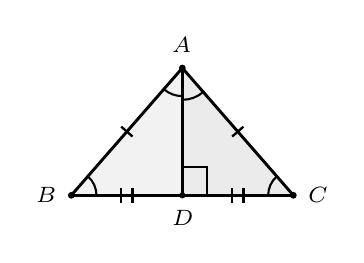
\begin{tikzpicture}[scale=0.94, every node/.style={font=\footnotesize, text=black}]
  \coordinate (A) at (0,1.72);
  \coordinate (B) at (-1.50,0);
  \coordinate (C) at (1.50,0);
  \coordinate (D) at (0,0);
  \fill[gray!10] (A) -- (B) -- (D) -- cycle;
  \fill[gray!16] (A) -- (D) -- (C) -- cycle;
  \draw[black, line width=1.05pt, tk1] (A) -- (B);
  \draw[black, line width=1.05pt, tk1] (A) -- (C);
  \draw[black, line width=1.0pt, tk2] (B) -- (D);
  \draw[black, line width=1.0pt, tk2] (D) -- (C);
  \draw[black, line width=1.05pt] (A) -- (D);
  \rightbox[0.22]{A}{D}{C}
  \draw[black, line width=0.75pt] ($(A)+(-131:0.38)$) arc (-131:-90:0.38);
  \draw[black, line width=0.75pt] ($(A)+(-90:0.43)$) arc (-90:-49:0.43);
  \draw[black, line width=0.75pt] ($(B)+(0:0.34)$) arc (0:49:0.34);
  \draw[black, line width=0.75pt] ($(C)+(180:0.34)$) arc (180:131:0.34);
  \fill[black] (A) circle (1.3pt) node[above=2pt] {$A$};
  \fill[black] (B) circle (1.3pt) node[left=2pt] {$B$};
  \fill[black] (C) circle (1.3pt) node[right=2pt] {$C$};
  \fill[black] (D) circle (1.2pt) node[below=2pt] {$D$};
\end{tikzpicture}}

% ៧. E3 Explain Inset: ប្រៀបធៀប ប្រសព្វពុះមុំ I (កែងជ្រុង ក្នុង) vs ប្រសព្វមេដ្យាទ័រ O (ស្មើកំពូល)
\newcommand{\figCenterContrastISO}{%
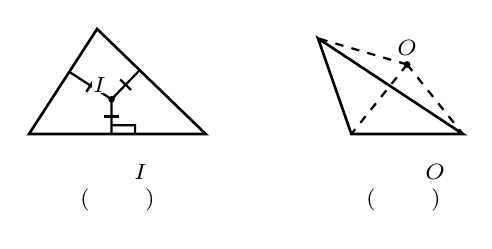
\begin{tikzpicture}[scale=0.92, every node/.style={font=\footnotesize, text=black}]
  % ឆ្វេង៖ ប្រសព្វពុះមុំ I (ស្មើចម្ងាយពីជ្រុង ៣, ក្នុងជានិច្ច)
  \begin{scope}[shift={(0,0)}]
    \coordinate (A) at (-0.28,1.45);
    \coordinate (B) at (-1.22,0);
    \coordinate (C) at (1.22,0);
    \coordinate (I) at (-0.08,0.48);
    \coordinate (D) at ($(A)!(I)!(B)$);
    \coordinate (E) at ($(B)!(I)!(C)$);
    \coordinate (F) at ($(A)!(I)!(C)$);
    \draw[black, line width=0.95pt] (A) -- (B) -- (C) -- cycle;
    \draw[black, line width=0.8pt, tk1] (I) -- (D);
    \draw[black, line width=0.8pt, tk1] (I) -- (E);
    \draw[black, line width=0.8pt, tk1] (I) -- (F);
    \rightbox[0.25]{I}{E}{C}
    \fill[black] (I) circle (1.3pt) node[above left=2pt, fill=white, inner sep=0.4pt] {$I$};
    \node[anchor=north, align=center] at (0,-0.28) {ពុះមុំ $I$\\(ស្មើជ្រុង)};
  \end{scope}
  % ស្ដាំ៖ ប្រសព្វមេដ្យាទ័រ O (ស្មើចម្ងាយពីកំពូល ៣)
  \begin{scope}[shift={(3.55,0)}]
    \coordinate (A) at (-0.78,1.32);
    \coordinate (B) at (-0.32,0);
    \coordinate (C) at (1.22,0);
    \coordinate (O) at (0.45,0.96);
    \draw[black, line width=0.95pt] (A) -- (B) -- (C) -- cycle;
    \draw[black, line width=0.8pt, dashed] (O) -- (A) (O) -- (B) (O) -- (C);
    \fill[black] (O) circle (1.3pt) node[above=2.5pt, fill=white, inner sep=0.4pt] {$O$};
    \node[anchor=north, align=center] at (0.40,-0.28) {មេដ្យាទ័រ $O$\\(ស្មើកំពូល)};
  \end{scope}
\end{tikzpicture}}

% ៨. E4 Elaborate: លំហាត់គំរូ (ទំ.១៥៧ កែតម្រូវ - △ABC មុំស្រួចមិនសមបាទ, 90° តែ L,M, គ្មាន 90° ត្រង់ N, ON ដាច់ៗ + ?)
\newcommand{\figModelISO}{%
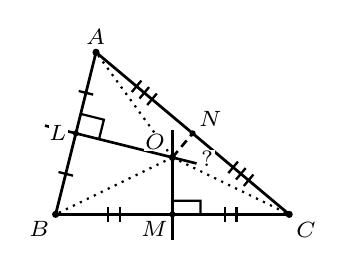
\begin{tikzpicture}[scale=1.00, every node/.style={font=\footnotesize, text=black}]
  \coordinate (O) at (0,0);
  \coordinate (A) at (-0.970, 1.335);
  \coordinate (B) at (-1.483,-0.723);
  \coordinate (C) at ( 1.483,-0.723);
  \coordinate (L) at (-1.226, 0.306);
  \coordinate (M) at ( 0.000,-0.723);
  \coordinate (N) at ( 0.257, 0.306);
  % សញ្ញាឆ្នូតលើកំណាត់ស្មើគ្នា AL=LB, BM=MC, AN=NC
  \draw[black, line width=1.0pt, tk1] (A) -- (L);
  \draw[black, line width=1.0pt, tk1] (L) -- (B);
  \draw[black, line width=1.0pt, tk2] (B) -- (M);
  \draw[black, line width=1.0pt, tk2] (M) -- (C);
  \draw[black, line width=1.0pt, tk3] (A) -- (N);
  \draw[black, line width=1.0pt, tk3] (N) -- (C);
  % មេដ្យាទ័រ L និង M ប្រសព្វត្រង់ O
  \draw[black, line width=0.95pt] ($(O)!-0.25!(L)$) -- ($(O)!1.32!(L)$);
  \draw[black, line width=0.95pt] (0,-1.05) -- (0,0.35);
  % កែង 90° តែត្រង់ L និង M ប៉ុណ្ណោះ (ហាមគូស 90° ត្រង់ N!)
  \rightbox[0.24]{O}{L}{A}
  \rightbox[0.24]{O}{M}{C}
  % ON ដាច់ៗ + ? និង OA, OB, OC ចុចៗសម្រាប់ [tracing]
  \draw[black, line width=0.95pt, densely dashed] (O) -- (N);
  \draw[black, line width=0.80pt, dotted] (O) -- (A) (O) -- (B) (O) -- (C);
  \fill[black] (A) circle (1.3pt) node[above=2pt, fill=white, inner sep=0.5pt] {$A$};
  \fill[black] (B) circle (1.3pt) node[below left=2pt, fill=white, inner sep=0.5pt] {$B$};
  \fill[black] (C) circle (1.3pt) node[below right=2pt, fill=white, inner sep=0.5pt] {$C$};
  \fill[black] (L) circle (1.1pt) node[left=2.5pt, fill=white, inner sep=0.4pt] {$L$};
  \fill[black] (M) circle (1.1pt) node[below left=2pt, fill=white, inner sep=0.4pt] {$M$};
  \fill[black] (N) circle (1.1pt) node[above right=2pt, fill=white, inner sep=0.4pt] {$N$};
  \fill[black] (O) circle (1.3pt) node[above left=2pt, fill=white, inner sep=0.5pt] {$O$};
  \node[fill=white, inner sep=0.4pt] at (0.45,-0.02) {$?$};
\end{tikzpicture}}

% ៩. E5 Evaluate: ប្រតិបត្តិ (ក) ហោជាង 50°, BC=10 m & (ខ) ប៉មទឹកផ្ទះ ៣ ខ្នងមុំទាល 110°, O ក្រៅ
\newcommand{\figPracticeISO}{%
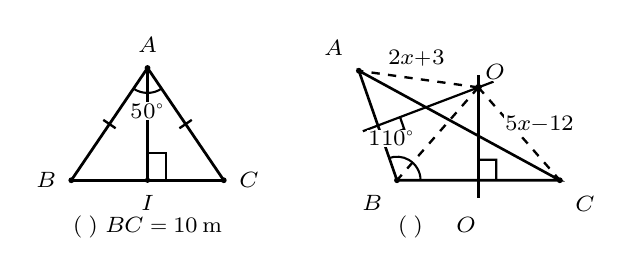
\begin{tikzpicture}[scale=0.88, every node/.style={font=\footnotesize, text=black}]
  % (ក) ហោជាង △ABC (AB=AC, ∠A=50°, AI⊥BC, BC=10 m)
  \begin{scope}[shift={(-2.35,0)}]
    \coordinate (A) at (0,1.62);
    \coordinate (B) at (-1.10,0);
    \coordinate (C) at (1.10,0);
    \coordinate (I) at (0,0);
    \draw[black, line width=1.0pt, tk1] (A) -- (B);
    \draw[black, line width=1.0pt, tk1] (A) -- (C);
    \draw[black, line width=1.0pt] (B) -- (C);
    \draw[black, line width=0.9pt] (A) -- (I);
    \rightbox[0.24]{A}{I}{C}
    \draw[black, line width=0.75pt] ($(A)+(-125:0.36)$) arc (-125:-55:0.36);
    \node[fill=white, inner sep=0.5pt] at (0,1.00) {$50^\circ$};
    \fill[black] (A) circle (1.2pt) node[above=2pt] {$A$};
    \fill[black] (B) circle (1.2pt) node[left=2pt] {$B$};
    \fill[black] (C) circle (1.2pt) node[right=2pt] {$C$};
    \fill[black] (I) circle (1.1pt) node[below=2pt] {$I$};
    \node at (0,-0.68) {(ក) $BC=10\unit{m}$};
  \end{scope}
  % (ខ) ផ្ទះ ៣ ខ្នង ∠B=110°, O ក្រៅ
  \begin{scope}[shift={(1.25,0)}]
    \coordinate (B) at (0,0);
    \coordinate (A) at (-0.55,1.58);
    \coordinate (C) at (2.35,0);
    \coordinate (O) at (1.175,1.34);
    \coordinate (L) at ($(A)!0.5!(B)$);
    \coordinate (M) at ($(B)!0.5!(C)$);
    \draw[black, line width=0.95pt] (A) -- (B) -- (C) -- cycle;
    \draw[black, line width=0.8pt] ($(L)!-0.15!(O)$) -- ($(L)!1.15!(O)$);
    \draw[black, line width=0.8pt] (1.175,-0.25) -- (1.175,1.52);
    \rightbox[0.22]{O}{L}{B}
    \rightbox[0.22]{O}{M}{C}
    \draw[black, line width=0.85pt, dashed] (O) -- (A) (O) -- (B) (O) -- (C);
    \draw[black, line width=0.75pt] ($(B)+(0:0.34)$) arc (0:110:0.34);
    \node[fill=white, inner sep=0.4pt] at (-0.08,0.60) {$110^\circ$};
    \fill[black] (A) circle (1.2pt) node[above left=2pt] {$A$};
    \fill[black] (B) circle (1.2pt) node[below left=2pt] {$B$};
    \fill[black] (C) circle (1.2pt) node[below right=2pt] {$C$};
    \fill[black] (O) circle (1.4pt) node[above right=2pt, fill=white, inner sep=0.5pt] {$O$};
    \node[fill=white, inner sep=0.4pt] at (0.28,1.76) {$2x{+}3$};
    \node[fill=white, inner sep=0.4pt] at (2.06,0.82) {$5x{-}12$};
    \node at (0.95,-0.68) {(ខ) ប៉ម $O$ ខាងក្រៅ};
  \end{scope}
\end{tikzpicture}}

% ១០. E5 Evaluate: កាតត្រួតពិនិត្យ A–D (ក្រឡា ២x២)
\newcommand{\figExitCardsISO}{%
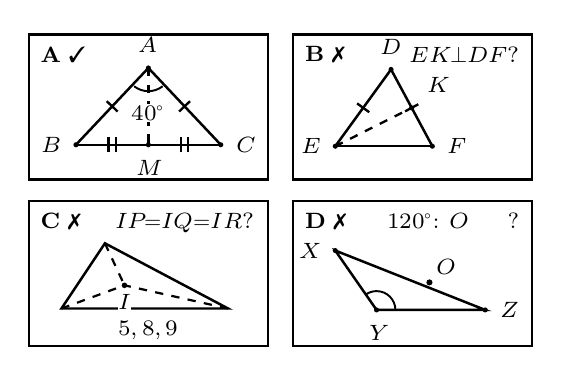
\begin{tikzpicture}[scale=0.92, every node/.style={font=\footnotesize, text=black}]
  % កាត A: AB=AC, ∠A=40°, BM=MC => AM⊥BC ✓
  \begin{scope}[shift={(0,2.30)}]
    \draw[black, line width=0.85pt] (0,0) rectangle (3.30,2.00);
    \node[anchor=north west, inner sep=3pt] at (0.04,1.96) {\textbf{A} \ding{51}};
    \coordinate (A) at (1.65,1.54);
    \coordinate (B) at (0.65,0.48);
    \coordinate (C) at (2.65,0.48);
    \coordinate (M) at (1.65,0.48);
    \draw[black, line width=0.9pt, tk1] (A) -- (B);
    \draw[black, line width=0.9pt, tk1] (A) -- (C);
    \draw[black, line width=0.9pt, tk2] (B) -- (M);
    \draw[black, line width=0.9pt, tk2] (M) -- (C);
    \draw[black, line width=0.85pt, dashed] (A) -- (M);
    \draw[black, line width=0.7pt] ($(A)+(-128:0.32)$) arc (-128:-52:0.32);
    \fill[black] (A) circle (1.0pt) node[above=2pt] {$A$};
    \fill[black] (B) circle (1.0pt) node[left=2pt] {$B$};
    \fill[black] (C) circle (1.0pt) node[right=2pt] {$C$};
    \fill[black] (M) circle (1.0pt) node[below=2pt] {$M$};
    \node[fill=white, inner sep=0.4pt] at (1.65,0.92) {$40^\circ$};
  \end{scope}
  % កាត B: Wrong-Apex Trap DE=DF=6, EF=4, មេដ្យាន EK ពី E ✗
  \begin{scope}[shift={(3.65,2.30)}]
    \draw[black, line width=0.85pt] (0,0) rectangle (3.30,2.00);
    \node[anchor=north west, inner sep=3pt] at (0.04,1.96) {\textbf{B} \ding{55}};
    \coordinate (D) at (1.35,1.52);
    \coordinate (E) at (0.58,0.46);
    \coordinate (F) at (1.92,0.46);
    \coordinate (K) at ($(D)!0.5!(F)$);
    \draw[black, line width=0.9pt, tk1] (D) -- (E);
    \draw[black, line width=0.9pt, tk1] (D) -- (F);
    \draw[black, line width=0.9pt] (E) -- (F);
    \draw[black, line width=0.85pt, dashed] (E) -- (K);
    \fill[black] (D) circle (1.0pt) node[above=2pt] {$D$};
    \fill[black] (E) circle (1.0pt) node[left=2pt] {$E$};
    \fill[black] (F) circle (1.0pt) node[right=2pt] {$F$};
    \fill[black] (K) circle (1.0pt) node[above right=2pt] {$K$};
    \node[anchor=north east, inner sep=3pt] at (3.24,1.96) {$EK{\perp}DF?$};
  \end{scope}
  % កាត C: 5,8,9 ពុះមុំ I vs IP=IQ=IR ✗
  \begin{scope}[shift={(0,0)}]
    \draw[black, line width=0.85pt] (0,0) rectangle (3.30,2.00);
    \node[anchor=north west, inner sep=3pt] at (0.04,1.96) {\textbf{C} \ding{55}};
    \coordinate (P) at (1.05,1.42);
    \coordinate (Q) at (0.45,0.52);
    \coordinate (R) at (2.75,0.52);
    \coordinate (I) at (1.32,0.84);
    \draw[black, line width=0.9pt] (P) -- (Q) -- (R) -- cycle;
    \draw[black, line width=0.8pt, dashed] (P) -- (I) (Q) -- (I) (R) -- (I);
    \fill[black] (I) circle (1.1pt) node[below=2.5pt, fill=white, inner sep=0.4pt] {$I$};
    \node[anchor=north east, inner sep=3pt] at (3.24,1.96) {$IP{=}IQ{=}IR?$};
    \node at (1.65,0.22) {$5, 8, 9$};
  \end{scope}
  % កាត D: មុំទាល 120°, O ខាងក្នុង? ✗
  \begin{scope}[shift={(3.65,0)}]
    \draw[black, line width=0.85pt] (0,0) rectangle (3.30,2.00);
    \node[anchor=north west, inner sep=3pt] at (0.04,1.96) {\textbf{D} \ding{55}};
    \coordinate (X) at (0.58,1.32);
    \coordinate (Y) at (1.15,0.50);
    \coordinate (Z) at (2.65,0.50);
    \coordinate (O) at (1.88,0.88);
    \draw[black, line width=0.9pt] (X) -- (Y) -- (Z) -- cycle;
    \draw[black, line width=0.7pt] ($(Y)+(0:0.26)$) arc (0:125:0.26);
    \fill[black] (X) circle (1.0pt) node[left=2pt] {$X$};
    \fill[black] (Y) circle (1.0pt) node[below=2pt] {$Y$};
    \fill[black] (Z) circle (1.0pt) node[right=2pt] {$Z$};
    \fill[black] (O) circle (1.2pt) node[above right=2pt, fill=white, inner sep=0.4pt] {$O$};
    \node[anchor=north east, inner sep=3pt] at (3.24,1.96) {$120^\circ$: $O$ ក្នុង?};
  \end{scope}
\end{tikzpicture}}

% ១១. ជំហានទី៥ កិច្ចការផ្ទះ៖ លំហាត់ទី២, ទី៨ និងទី១១ (ទំ.១៦៤--១៦៥)
\newcommand{\figHWnewISO}{%
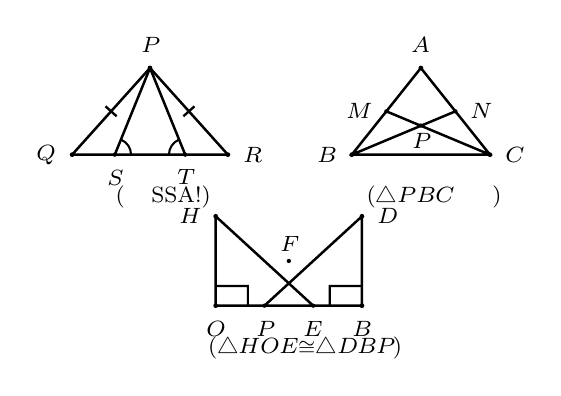
\begin{tikzpicture}[scale=0.86, every node/.style={font=\footnotesize, text=black}]
  % លំហាត់ទី២ (ទំ.១៦៤ - ជួរលើឆ្វេង)
  \begin{scope}[shift={(-2.05,1.88)}]
    \coordinate (P) at (0,1.28);
    \coordinate (Q) at (-1.15,0);
    \coordinate (R) at (1.15,0);
    \coordinate (S) at (-0.52,0);
    \coordinate (T) at (0.52,0);
    \draw[black, line width=0.9pt, tk1] (P) -- (Q);
    \draw[black, line width=0.9pt, tk1] (P) -- (R);
    \draw[black, line width=0.9pt] (Q) -- (R) (P) -- (S) (P) -- (T);
    \draw[black, line width=0.75pt] ($(S)+(0:0.24)$) arc (0:67:0.24);
    \draw[black, line width=0.75pt] ($(T)+(180:0.24)$) arc (180:113:0.24);
    \fill[black] (P) circle (1.0pt) node[above=2pt] {$P$};
    \fill[black] (Q) circle (1.0pt) node[left=2pt] {$Q$};
    \fill[black] (R) circle (1.0pt) node[right=2pt] {$R$};
    \fill[black] (S) circle (0.9pt) node[below=2pt] {$S$};
    \fill[black] (T) circle (0.9pt) node[below=2pt] {$T$};
    \node at (0,-0.62) {ទី២ (ហាម \en{SSA!})};
  \end{scope}
  % លំហាត់ទី៨ (ទំ.១៦៥ - ជួរលើស្ដាំ)
  \begin{scope}[shift={(1.95,1.88)}]
    \coordinate (A) at (0,1.28);
    \coordinate (B) at (-1.02,0);
    \coordinate (C) at (1.02,0);
    \coordinate (M) at ($(A)!0.5!(B)$);
    \coordinate (N) at ($(A)!0.5!(C)$);
    \coordinate (P) at (0,0.43);
    \draw[black, line width=0.9pt] (A) -- (B) -- (C) -- cycle (B) -- (N) (C) -- (M);
    \fill[black] (A) circle (1.0pt) node[above=2pt] {$A$};
    \fill[black] (B) circle (1.0pt) node[left=2pt] {$B$};
    \fill[black] (C) circle (1.0pt) node[right=2pt] {$C$};
    \fill[black] (M) circle (0.9pt) node[left=2pt] {$M$};
    \fill[black] (N) circle (0.9pt) node[right=2pt] {$N$};
    \fill[black] (P) circle (0.9pt) node[below=2.5pt, fill=white, inner sep=0.3pt] {$P$};
    \node at (0,-0.62) {ទី៨ ($\tri{PBC}$ សមបាទ)};
  \end{scope}
  % លំហាត់ទី១១ (ទំ.១៦៥ - ជួរក្រោមកណ្ដាល)
  \begin{scope}[shift={(0,-0.35)}]
    \coordinate (O) at (-1.08,0);
    \coordinate (B) at (1.08,0);
    \coordinate (P) at (-0.36,0);
    \coordinate (E) at (0.36,0);
    \coordinate (H) at (-1.08,1.32);
    \coordinate (D) at (1.08,1.32);
    \coordinate (F) at (0,0.66);
    \draw[black, line width=0.9pt] (H) -- (O) -- (B) -- (D) (H) -- (E) (D) -- (P);
    \rightbox[0.22]{H}{O}{B}
    \rightbox[0.22]{D}{B}{O}
    \fill[black] (H) circle (1.0pt) node[left=2pt] {$H$};
    \fill[black] (D) circle (1.0pt) node[right=2pt] {$D$};
    \fill[black] (O) circle (1.0pt) node[below=2pt] {$O$};
    \fill[black] (P) circle (0.9pt) node[below=2pt] {$P$};
    \fill[black] (E) circle (0.9pt) node[below=2pt] {$E$};
    \fill[black] (B) circle (1.0pt) node[below=2pt] {$B$};
    \fill[black] (F) circle (0.9pt) node[above=3pt, fill=white, inner sep=0.4pt] {$F$};
    \node at (0,-0.62) {ទី១១ ($\tri{HOE}{\cg}\tri{DBP}$)};
  \end{scope}
\end{tikzpicture}}

% ============================================================================
% ចាប់ផ្ដើមឯកសារ (Document Body)
% ============================================================================
\begin{document}
\fontsize{10pt}{15.2pt}\selectfont

% -------------------- ក្បាលកិច្ចតែងការ (Header) --------------------
\begin{center}
  {\muol\fontsize{11pt}{16pt}\selectfont ព្រះរាជាណាចក្រកម្ពុជា}\\[2pt]
  {\muol\fontsize{10pt}{15pt}\selectfont ជាតិ សាសនា ព្រះមហាក្សត្រ}\\[1pt]
  \khmflourish
\end{center}

\vspace{-15pt}
{\muol\fontsize{9.5pt}{13.2pt}\selectfont
មន្ទីរអប់រំ យុវជន និងកីឡា ខេត្តកំពង់ធំ\\
ការិយាល័យអប់រំ យុវជន និងកីឡា ស្រុកកំពង់ស្វាយ\\
អនុវិទ្យាល័យព្រះក្រសាំង}

\vspace{2pt}
\begin{center}
  {\muol\fontsize{10pt}{15pt}\selectfont កិច្ចតែងការបង្រៀន}
\end{center}
\vspace{1pt}

% -------------------- ព័ត៌មានទូទៅ (Metadata) --------------------
{\renewcommand{\arraystretch}{1.04}
\hspace*{4.05cm}%
\begin{tabular}{@{}l l l@{}}
  - \hspace{0.35cm} មុខវិជ្ជា & : & គណិតវិទ្យា ថ្នាក់ទី៨ \\
  - \hspace{0.35cm} ចំណងជើងមេរៀន & : & មេរៀនទី១២ ការប្រៀបធៀបត្រីកោណ \\
  - \hspace{0.35cm} ចំណងជើងរង & : & ២. មេដ្យាទ័រនៃអង្កត់និងត្រីកោណសមបាទ \\
  & & ២.២ លក្ខណៈត្រីកោណសមបាទ និងប្រសព្វមេដ្យាទ័រ \\
  - \hspace{0.35cm} រយៈពេល & : & ១ ម៉ោងសិក្សា (៥០នាទី) \\
  - \hspace{0.35cm} បង្រៀនដោយ & : & ហុក ប៊ុនថែន \\
  - \hspace{0.35cm} កាលបរិច្ឆេទ & : & ថ្ងៃពុធ ទី២ ខែធ្នូ ឆ្នាំ២០២៦ \\
\end{tabular}

\vspace{2pt}

% -------------------- I. វត្ថុបំណង --------------------
\textbf{I.} {\muol វត្ថុបំណង}\\[2pt]
\hspace*{0.55cm}%
\begin{tabular}{@{}l l l@{}}
  \wcirc \hspace{0.25cm} វិជ្ជាសម្បទា & : & សិស្សប្រាប់និងស្រាយបញ្ជាក់លក្ខណៈផ្ទាល់-ច្រាសត្រីកោណសមបាទ (ជ.ម.ជ / ម.ជ.ម) បន្ទាត់រួម ៤-ក្នុង-១ \\
  & & ចេញពីកំពូល និងប្រសព្វមេដ្យាទ័រ $O$ ($OA=OB=OC$) ក្នុងត្រីកោណមុំស្រួច (ក្នុង) និងមុំទាល (ក្រៅ) ។ \\
  \wcirc \hspace{0.25cm} បំណិនសម្បទា & : & សិស្សបត់ក្រដាស $1:1$ ($BC=6.0\text{ cm}, AB=AC=5.0\text{ cm}$) ធៀបរូបកំពូលខុស ($\tri{PQR}$) ធ្វើ POE \\
  & & ប្រើ \textbf{[tracing]} និង \cnum{1}--\cnum{5} ស្រាយ $ON\perp AC$ និងដោះស្រាយបញ្ហាហោជាង-ប៉មទឹក ($x=5, 13\text{ m}$) ។ \\
  \wcirc \hspace{0.25cm} ចរិយាសម្បទា & : & សិស្សសហការជា «ក្រុមស្ថាបត្យករហោជាង និងប៉មទឹកសហគមន៍» ចៀសវាងអន្ទាក់កំពូលខុស \\
  & & ប្រយ័ត្នការច្រឡំ $O$ នឹង $I$ និងអន្ទាក់ \en{SSA} តាមវិន័យពិភាក្សា \en{Pause-Ask / Pause-Review} ។ \\
\end{tabular}

\vspace{2pt}

% -------------------- II. សម្ភារៈឧបទេស --------------------
\textbf{II.} {\muol សម្ភារៈឧបទេស}\\[2pt]
\hspace*{0.55cm}$\bullet$ \hspace{0.35cm} សៀវភៅគោលទី៨ (ទំ.១៥៧--១៥៨, ១៦៤--១៦៥) បន្ទាត់ក្រិត ១:១ រ៉ាព័រទ័រ ដែកឈាន កន្ត្រៃ កញ្ចប់ ១:១ (ទំព័រ ១) កាត E4 (ទំព័រ ២) សន្លឹក E5 (ទំព័រ ៣) ផ្ទាំង \cnum{1}--\cnum{5} (ទំព័រ ៤) កាត A--D (ទំព័រ ៥) និងប័ណ្ណកិច្ចការផ្ទះ (ទំព័រ ៦)

\vspace{2pt}

% -------------------- III. វិធីសាស្រ្តបង្រៀន --------------------
\textbf{III.} {\muol វិធីសាស្រ្តបង្រៀន}\\[2pt]
\hspace*{0.55cm}%
\begin{tabular}{@{}l l l@{}}
  $\bullet$ \hspace{0.35cm} គោលវិធី & : \hspace{0.7cm} & សិស្សមជ្ឈមណ្ឌល \\
  $\bullet$ \hspace{0.35cm} យុទ្ធវិធីបង្រៀន & : & ស្ថាបនានិយម គម្រូ 5Es (បត់ក្រដាស ១:១ កំពូលខុស POE មុំស្រួច-ទាល \textbf{[tracing]} \& ៣ តួនាទី) \\
\end{tabular}
}

\vspace{2pt}

% -------------------- IV. ដំណើរការបង្រៀន --------------------
\textbf{IV.} {\muol ដំណើរការបង្រៀន}

\vspace{-3pt}

% ============================================================================
% តារាងដំណើរការបង្រៀន (Modular Multi-Row 3-Column Table – 50 នាទី)
% ============================================================================
\renewcommand{\arraystretch}{1.15}
\begin{longtable}{|L{5.50cm}|L{7.90cm}|L{4.80cm}|}
\hline
\rowcolor{headgray}
\multicolumn{1}{|c|}{\muol សកម្មភាពគ្រូ} &
\multicolumn{1}{c|}{\muol ខ្លឹមសារមេរៀន} &
\multicolumn{1}{c|}{\muol សកម្មភាពសិស្ស} \\
\hline
\endfirsthead

\hline
\endhead

\hline
\endfoot

\hline
\endlastfoot

% ==================== ជំហានទី១ (2min) ====================
\stepheader{ជំហានទី១ \enbf{(}រដ្ឋបាលថ្នាក់\enbf{)}}
$\bullet$ ពិនិត្យអវត្តមាន និងអនាម័យថ្នាក់រៀន\par
$\bullet$ ចាត់ក្រុម ៣ នាក់ («ក្រុមស្ថាបត្យករហោជាង និងប៉មទឹកសហគមន៍»)\par
$\bullet$ ចែកកញ្ចប់ ១:១ (ទំព័រ ១) ដាក់ផ្កាប់លើតុ
&
\hspace*{0.3cm}-- រដ្ឋបាលថ្នាក់\par
\hspace*{0.3cm}-- អនាម័យ និងសណ្ដាប់ធ្នាប់ថ្នាក់រៀន\par
\hspace*{0.3cm}-- ត្រៀមក្រុមស្ថាបត្យករហោជាង និងប៉មទឹកសហគមន៍
&
\wcirc\ រាយការណ៍អវត្តមាន\par
\wcirc\ អង្គុយតាមក្រុម ៣ នាក់ \\
\hline

% ==================== ជំហានទី២ (9min: HW 3m + Prereq 3m + E1 3m) ====================
\stepheader{ជំហានទី២ \enbf{(}កិច្ចការផ្ទះ \enbf{+} ទំនាក់ទំនងមេរៀនថ្មី\enbf{)}}
% --- ២.១ កំណែកិច្ចការផ្ទះ ---
$\bullet$ ពិនិត្យកិច្ចការផ្ទះ (លំហាត់ទី១, ទី៣, ទី៥ ទំ.១៦៤)\par
\timenote{ចំណាយពេលឱ្យតិចបំផុតកុំឱ្យលើស 3min}\par
– \textbf{សំណួរបញ្ឆោត៖} «ក្នុងលំហាត់ទី៥(ខ) ហេតុអ្វីគ្រាន់តែ $T$ ជាចំណុចកណ្ដាលនៃ $RS$ មិនទាន់គ្រប់ធ្វើឱ្យបន្ទាត់ជាមេដ្យាទ័រទេ?»
&
\centerline{\redsub{កំណែកិច្ចការផ្ទះ (លំហាត់ទី១, ទី៣, ទី៥ ទំ.១៦៤)}}
&
\wcirc\ ផ្ទៀងកិច្ចការផ្ទះតាមក្រុម \\[3pt]
& \cfig{\figHWoldISO} & \\[3pt]
$\bullet$ សម្របសម្រួលសិស្សបញ្ជាក់លក្ខខណ្ឌកែង $90^\circ$
&
\textbf{ទី១៖} $\tri{ABC}\cg\tri{DEF} \Rightarrow 2x+30=5x-90 \Rightarrow x=40,\ BC=110\unit{cm}$\par
\textbf{ទី៣៖} $MT=MB, MA=MO$ និងមុំរួម $\ang{M} \Rightarrow \tri{MTO}\cg\tri{MBA}$ (ជ.ម.ជ)\par
\textbf{ទី៥៖} \textbf{(ក)} $AB\parallel CD, TR=TS \Rightarrow \tri{ABT}\cg\tri{DCT}$\par
\hspace*{0.2cm}\textbf{(ខ)} $\Delta\perp RS$ កាត់ $T$ \graybox{ត្រូវមានសោទី២ គឺកែង $90^\circ$ ត្រង់ $T$}
&
\wcirc\ ឆ្លើយ៖ «ត្រូវមានសោទី២ គឺកែង $90^\circ$ ត្រង់ $T$ ទើបជាមេដ្យាទ័រ!» \\[3pt]

% --- ២.២ រំលឹកមេរៀនទាក់ទង (3min) ---
\ditem \textbf{រំលឹករហ័ស} \timenote{(សរុបកុំឱ្យលើស 3min)}\par
– \textbf{សំណួរ៖} ប្រាប់ឈ្មោះផ្នែកនៃត្រីកោណសមបាទ ($\tri{ABC}, AB=AC$)\par
– \textbf{សំណួរ៖} ញែកមេដ្យាន កម្ពស់ ពុះមុំ និងមេដ្យាទ័រ + ទ្រឹស្ដីបទមេដ្យាទ័រ (២.១)
&
\centerline{\redsub{រំលឹកមេរៀនទាក់ទងមេរៀនថ្មី}}
&
\wcirc\ គិតរំលឹកវាក្យសព្ទត្រីកោណសមបាទ និងបន្ទាត់ពិសេស \\[3pt]
& \cfig{\figPrereqISO} & \\[3pt]
$\bullet$ បញ្ជាក់ភាពខុសគ្នារវាងមេដ្យាន កម្ពស់ ពុះមុំ និងមេដ្យាទ័រ
&
\hspace*{0.2cm}-- ត្រីកោណសមបាទ៖ កំពូល $A$, ជ្រុងស្មើ $AB=AC$, បាទ $BC$, មុំបាទ $\ang{B}, \ang{C}$\par
\hspace*{0.2cm}-- មេដ្យាន (កំពូល$\to$កណ្ដាល) $\vert$ កម្ពស់ (កំពូល$\to 90^\circ$) $\vert$ ពុះមុំ $\vert$ មេដ្យាទ័រ ($\perp$ កណ្ដាល)\par
\hspace*{0.2cm}-- ទ្រឹស្ដីបទ ២.១ (ផ្ទាល់-ច្រាស)៖ $M\in\Delta \Leftrightarrow MB=MC$
&
\wcirc\ ឆ្លើយ៖ «កំពូល $A$, បាទ $BC$, មេដ្យាទ័រមិនបាច់កាត់កំពូល; $M\in\Delta \Leftrightarrow MB=MC$!» \\[3pt]

% --- ២.៣ E1 Engage: ហោជាងសាលាឆទាន និងប៉មទឹកសហគមន៍ ---
\fiveE{E1 - Engage (3min)}\par
\ditem \textbf{ហោជាងសាលាឆទាន និងប៉មទឹកសហគមន៍ស្មើចម្ងាយពីផ្ទះ ៣ ខ្នង៖}\par
\hspace*{0.1cm}(១) ខ្សែប្រយោលកែង $90^\circ$ ពីកំពូល $A$ នៃហោជាង $\tri{ABC}$ ($AB=AC$) ប៉ះកណ្ដាល $I$ ($IB=IC$) និងពុះ $\ang{A}$ ស្មើគ្នា — ហេតុអ្វីខ្សែ ៤ ក្លាយជា ១?\par
\hspace*{0.1cm}(២) ផ្ទះ ៣ ខ្នង $A,B,C$ រកប៉មទឹក $O$ ឱ្យ $OA=OB=OC$ — រកដូចម្ដេច ហើយ $O$ នៅក្នុងឬក្រៅ?
&
\centerline{\redsub{ស្ថានភាពពិត៖ ហោជាងសាលាឆទាន និងប៉មទឹកផ្ទះ ៣ ខ្នង}}
&
\wcirc\ សង្កេតរូបហោជាងសាលាឆទាន និងផ្ទះ ៣ ខ្នង \\[3pt]
& \cfig{\figEngageISO} & \\[3pt]
– \textbf{សំណួរ៖} តើ $O$ ស្ថិតនៅខាងក្នុង $\tri{ABC}$ ជានិច្ចឬទេ?
&
\textbf{ចម្ងល់៖}\par
\hspace*{0.2cm}(១) ហេតុអ្វីបន្ទាត់ ៤ រលាយជាខ្សែ ១?\par
\hspace*{0.2cm}(២) តើ $O$ នៅក្នុង $\tri{ABC}$ ជានិច្ចឬទេ?
&
\wcirc\ ទស្សន៍ទាយមូលហេតុបន្ទាត់ ៤-ក្នុង-១ និងទីតាំង $O$ ក្នុងឬក្រៅត្រីកោណ \\
\hline

% ==================== ជំហានទី៣ (17min: E2 11m + E3 6m) ====================
\stepheader{ជំហានទី៣ \enbf{(}ខ្លឹមសារមេរៀនថ្មី\enbf{)}}
% --- ៣.១ ចំណងជើង & E2 Act 1 (6min) ---
\fiveE{E2 - Explore (11min)}\par
$\bullet$ សរសេរចំណងជើងមេរៀនលើក្ដារខៀន\par
\ditem \textbf{សកម្មភាព ១៖ បត់ ១:១ (6min)}\par
– ផ្ទៀងក្រិត $5.0\unit{cm}$ (\en{Actual Size 100\%}, ទំព័រ ១) កាត់ $\tri{ABC}$ ($BC=6.0, AB=AC=5.0, AI=4.0\unit{cm}$) បត់ $B\mapsto C$ តាម $(AI)$\par
– ធៀបនឹងរូបកំពូលខុស $\tri{PQR}$ ($PQ=PR=4.5, QR=3.0\unit{cm}$) វាស់ពីកំពូលបាទ $Q$!
&
មេរៀនទី១២ \hspace{0.1cm} {\muol ការប្រៀបធៀបត្រីកោណ} \textbf{(ត)}\par
២. មេដ្យាទ័រនៃអង្កត់និងត្រីកោណសមបាទ\par
២.២ លក្ខណៈត្រីកោណសមបាទ និងប្រសព្វមេដ្យាទ័រ
&
\wcirc\ កត់ចំណងជើងមេរៀន\par
\wcirc\ ផ្ទៀងក្រិត $5.0\unit{cm}$ និងកាត់រូប $\tri{ABC}$ \\[3pt]
& \cfig{\figExploreOneISO} & \\[3pt]
$\bullet$ ប្រមូលលទ្ធផលបត់ និងវាស់គម្លាតកំពូលខុស $Q$
&
\hspace*{0.2cm}-- $\tri{ABC}$៖ បត់ $B\mapsto C \Rightarrow \ang{B}=\ang{C}, IB=IC=3.0\unit{cm}, \ang{AIB}=90^\circ, \ang{BAI}=\ang{CAI}$ (\graybox{៤-ក្នុង-១!})\par
\hspace*{0.2cm}-- កំពូលខុស $Q$ នៃ $\tri{PQR}$៖ មេដ្យាន $QM$ ($PM=MR=2.25, \ang{QMR}\approx 66^\circ\neq 90^\circ$) $\neq$ កម្ពស់ $QH\perp PR$ ($PH=3.50, HR=1.00$, គម្លាត $MH=1.25\unit{cm}$) ព្រោះ $QP=4.5\neq QR=3.0\unit{cm}$!
&
\wcirc\ បត់ $B\mapsto C$ ផ្ទៀង $4$-ក្នុង-$1$ និងវាស់បដិសេធកំពូលខុស $Q$ លើ $\tri{PQR}$ \\[3pt]

% --- ៣.២ E2 Act 2 POE (5min) ---
\ditem \textbf{សកម្មភាព ២៖ POE ប្រសព្វមេដ្យាទ័រ (5min)}\par
– \textbf{Panel A (មុំស្រួច $\tri{ABC}$)}៖ គូសមេដ្យាទ័រ $AB, BC$ ជួបគ្នាត្រង់ $O$ វាស់ $OA, OB, OC$\par
– \textbf{Panel B (មុំទាល $\tri{DEF}, \ang{E}=115^\circ$)}៖ ទាយទីតាំង $O'$ បន្លាយមេដ្យាទ័រ $DE, EF$ រួចវាស់ $O'D, O'E, O'F$
&
{\centering\textbf{POE៖ Panel A (មុំស្រួច $O$ ក្នុង) vs Panel B (មុំទាល $115^\circ$ $O'$ ក្រៅ)}\par}
&
\wcirc\ ទាយទីតាំង $O$ និង $O'$ មុនគូសបន្ទាត់ \\[3pt]
& \cfig{\figExploreTwoISO} & \\[3pt]
– \textbf{សំណួរ៖} ហេតុអ្វី $O$ នៅខាងក្នុងមុំស្រួច តែ $O'$ លោតទៅខាងក្រៅត្រីកោណមុំទាល?
&
\hspace*{0.2cm}-- \textbf{Panel A} ($\ang{A}=75^\circ, \ang{B}=61^\circ, \ang{C}=44^\circ$)៖ $O$ នៅ\textbf{ខាងក្នុង} (មិនកាត់កំពូលឈម), $OA=OB=OC=3.0\unit{cm}$\par
\hspace*{0.2cm}-- \textbf{Panel B} ($\ang{E}=115^\circ>90^\circ$)៖ $O'$ នៅ\textbf{ខាងក្រៅ}ឈម $\ang{E}$, តែបន្ទាត់/រង្វង់ផ្ទៀង $O'D=O'E=O'F=3.0\unit{cm}$!
&
\wcirc\ ទាយ-សង្កេត-ពន្យល់៖ មុំស្រួច $O$ ក្នុង vs មុំទាល $O'$ ក្រៅ តែស្មើចម្ងាយពីកំពូល ៣ \\[3pt]

% --- ៣.៣ E3 Explain: លក្ខណៈផ្ទាល់ ច្រាស (ម.ជ.ម) និង ៤-ក្នុង-១ (ទំ.១៥៧) ---
\fiveE{E3 - Explain (6min)}\par
\ditem បង្គុំលក្ខណៈ\textbf{ផ្ទាល់} ($AB=AC\Rightarrow\ang{B}=\ang{C}$) \textbf{ច្រាស} ($\ang{B}=\ang{C}\Rightarrow AB=AC$ តាម \textbf{ម.ជ.ម}) និង \textbf{៤-ក្នុង-១} (ទំ.១៥៧)\par
\timenote{(បំពេញ «។» ចុងបន្ទាត់លក្ខណៈទី១ និងសម្រួល «ស្ថិតនៅលើ»)}
&
\textbf{លក្ខណៈត្រីកោណសមបាទ (ទំ.១៥៧ + ច្រាស)៖}
&
\wcirc\ កត់ចំណងជើងលក្ខណៈត្រីកោណសមបាទ \\[3pt]
& \cfig{\figExplainISO} & \\[3pt]
$\bullet$ សង្កត់ធ្ងន់សម្រាយច្រាស ២ បន្ទាត់តាម \textbf{ម.ជ.ម / ASA} និងបន្ទាត់ ៤-ក្នុង-១
&
\textbf{(ផ្ទាល់)} $AB=AC \Rightarrow$ មុំបាទ $\ang{B}=\ang{C}$ \textbf{។}\par
\hspace*{0.2cm}(តាមពុះមុំ $AD$: $\tri{ABD}\cg\tri{ACD}$ ជ.ម.ជ)\par
\textbf{(ច្រាស $\ang{B}=\ang{C}\Rightarrow AB=AC$)}\par
\hspace*{0.2cm}-- គូសពុះមុំ $AD$ នៃ $\ang{A}$ ($\ang{BAD}=\ang{CAD}$)\par
\hspace*{0.2cm}-- តាម $180^\circ$, $\ang{ADB}=\ang{ADC}$; ជ្រុងរួម $AD$\par
\hspace*{0.2cm}$\Rightarrow \tri{ABD}\cg\tri{ACD}$ (\graybox{ម.ជ.ម / ASA}) $\Rightarrow AB=AC$ ។\par
\textbf{(៤-ក្នុង-១ ចេញពីកំពូល $A$ ប៉ុណ្ណោះ)}\par
មេដ្យាទ័រ មេដ្យាន កម្ពស់គូសចេញពីកំពូល និងកន្លះបន្ទាត់ពុះនៃមុំកំពូលនោះ \textbf{ស្ថិតនៅលើ}បន្ទាត់តែមួយ ។
&
\wcirc\ កត់លក្ខណៈផ្ទាល់ សម្រាយច្រាស ២ បន្ទាត់ (ម.ជ.ម) និង ៤-ក្នុង-១ (ពីកំពូលតែ ១) \\[3pt]

% --- ៣.៤ E3 Explain: ប្រសព្វមេដ្យាទ័រ (ទំ.១៥៨) កែអក្ខរាវិរុទ្ធ & ធនាគារ ①–⑤ ---
\cnum{1} បង្គុំទ្រឹស្ដីប្រសព្វមេដ្យាទ័រ (ទំ.១៥៨)\par
\timenote{(កែខុសទំ.១៥៧ «មេដ្យានទ័រ»$\to$«មេដ្យាទ័រ» និង «ស្ថិតនៅស្មើ»)}
&
\textbf{ទ្រឹស្ដីបទប្រសព្វមេដ្យាទ័រ (ទំ.១៥៨)៖}\par
មេដ្យាទ័រជ្រុងទាំងបីនៃត្រីកោណមួយប្រសព្វគ្នាត្រង់ចំណុចតែមួយ ($O$) ដែល\textbf{ស្ថិតនៅស្មើ}ចម្ងាយពីកំពូលទាំងបី ($OA=OB=OC$) ។
&
\wcirc\ កត់ទ្រឹស្ដីប្រសព្វ និងកែពាក្យ «មេដ្យាទ័រ» \\[3pt]
& \cfig{\figCenterContrastISO} & \\[3pt]
\cnum{2} ញែក \textbf{ប្រសព្វពុះមុំ $I$ vs ប្រសព្វមេដ្យាទ័រ $O$}
&
{\centering\renewcommand{\arraystretch}{1.10}%
\begin{tabular}{|L{3.50cm}|L{3.70cm}|}
  \hline
  \cellcolor{headgray}\centering\textbf{ប្រសព្វពុះមុំ $I$} & \cellcolor{headgray}\centering\arraybackslash\textbf{ប្រសព្វមេដ្យាទ័រ $O$} \\
  \hline
  ស្មើចម្ងាយពីជ្រុង ៣\par ក្នុងត្រីកោណជានិច្ច & ស្មើចម្ងាយពីកំពូល ៣\par ក្នុង (ស្រួច) / ក្រៅ (ទាល) \\
  \hline
\end{tabular}\par}
&
\wcirc\ ញែកលក្ខណៈខុសគ្នារវាង $I$ និង $O$ \\[3pt]

\cnum{3} បិទផ្ទាំង \textbf{ធនាគារ \cnum{1}--\cnum{5}} (ទំព័រ ៤)
&
\textbf{ធនាគារហេតុផល \cnum{1}--\cnum{5}៖}\par
\cnum{1} លក្ខណៈផ្ទាល់ត្រីកោណសមបាទ ($AB=AC\Rightarrow\ang{B}=\ang{C}$)\par
\cnum{2} លក្ខណៈច្រាសត្រីកោណសមបាទ ($\ang{B}=\ang{C}\Rightarrow AB=AC$)\par
\cnum{3} បន្ទាត់រួម ៤-ក្នុង-១ ចេញពីកំពូលត្រីកោណសមបាទ (មេដ្យាទ័រ$\equiv$មេដ្យាន$\equiv$កម្ពស់$\equiv$ពុះមុំកំពូល)
&
\wcirc\ កត់ធនាគារ \cnum{1}--\cnum{3} ទុកប្រើក្នុងសម្រាយ \\[3pt]
&
\cnum{4} ទ្រឹស្ដីបទមេដ្យាទ័រ និងប្រសព្វមេដ្យាទ័រទាំងបី ($OA=OB=OC$)\par
\cnum{5} លក្ខខណ្ឌត្រីកោណប៉ុនគ្នា (ម.ជ.ម/ជ.ម.ជ/ជ.ជ.ជ) និងផលបូកមុំ $180^\circ$ ។
&
\wcirc\ កត់ធនាគារ \cnum{4}--\cnum{5} ទុកប្រើក្នុងសម្រាយ \\
\hline

% ==================== ជំហានទី៤ (20min: E4 10m + E5 10m) ====================
\stepheader{ជំហានទី៤ \enbf{(}ពង្រីកចំណេះដឹង\enbf{)}}
% --- ៤.១ E4 Elaborate: កាត ផែនទីច្រវាក់ប្រសព្វមេដ្យាទ័រ (ទំព័រ ២) ---
\fiveE{E4 - Elaborate (10min)}\par
\ditem ចែកកាត \textbf{«ផែនទីច្រវាក់ប្រសព្វមេដ្យាទ័រ និងបន្ទាត់ ៤-ក្នុង-១»} (ទំព័រ ២)៖\par
\hspace*{0.1cm}\cnum{1} ពិនិត្យ $\tri{ABC}$ មុំស្រួចមិនសមបាទ (គ្មាន $90^\circ$ ត្រង់ $N$) និង \textbf{[tracing]} លើ $OA, OB, OC$
&
{\muol លំហាត់គំរូ} \textbf{(ទំ.១៥៧ កែតម្រូវ) ៖}\par
មេដ្យាទ័រនៃ $AB, BC$ នៃ $\tri{ABC}$ ប្រសព្វត្រង់ $O$ ។\par
\hspace*{0.15cm}ក. បង្ហាញថា $OA=OB=OC$ ។\par
\hspace*{0.15cm}ខ. បើ $N$ ចំណុចកណ្ដាល $AC$ បង្ហាញថា $ON\perp AC$ ។
&
\wcirc\ អានប្រធាន និងគូស \textbf{[tracing]} លើ $OA, OB, OC$ \\[3pt]
& \cfig{\figModelISO} & \\[3pt]
\hspace*{0.1cm}\cnum{2} ស្រាយ \textbf{(ក)} $OA=OB=OC$ និង \textbf{(ខ)} $ON\perp AC$ + \textbf{EIA 30s}
&
\textbf{ក. បង្ហាញ $OA=OB=OC$៖}\par
\hspace*{0.2cm}-- $O$ លើមេដ្យាទ័រ $AB \Rightarrow OA=OB$ (\cnum{4})\par
\hspace*{0.2cm}-- $O$ លើមេដ្យាទ័រ $BC \Rightarrow OB=OC$ (\cnum{4})\par
\hspace*{0.2cm}$\Rightarrow$ \graybox{$OA=OB=OC$} ។\par
\textbf{ខ. បង្ហាញ $ON\perp AC$៖}\par
\hspace*{0.2cm}-- ពី $OA=OC \Rightarrow \tri{OAC}$ សមបាទកំពូល $O$\par
\hspace*{0.2cm}-- ដោយ $N$ កណ្ដាល $AC$, $ON$ ជាមេដ្យានចេញពីកំពូល $O$\par
\hspace*{0.2cm}$\Rightarrow$ \graybox{$ON\perp AC$} (\cnum{3} បន្ទាត់ ៤-ក្នុង-១) ។\par
\timenote{EIA 30s៖ ហេតុអ្វី $ON$ មិនកាត់កំពូល $B$? (ព្រោះ $BA\neq BC$ — មេដ្យាទ័រ $AC$ មិនមែនមេដ្យាន $BN$ ទេ!)}
&
\wcirc\ សរសេរសម្រាយ (ក)-(ខ) ប្រើ \cnum{4}, \cnum{3} និងឆ្លើយ EIA 30s \\[3pt]

% --- ៤.២ E5 Evaluate: ប្រតិបត្តិ (6.5min, ទំព័រ ៣) ---
\fiveE{E5 - Evaluate (10min)}\par
\ditem {\muol លំហាត់ប្រតិបត្តិ} \textbf{(6.5min, ទំព័រ ៣)}\par
ចែកសន្លឹក \textbf{«តុផ្ទៀងផ្ទាត់មុំបាទ និងប៉មទឹកសហគមន៍ ៣ តួនាទី»} (\en{Pause-Ask / Pause-Review})៖\par
\hspace*{0.05cm}\cnum{1} តួនាទី ១ (\en{Pause-Ask})៖ ផ្ទៀង ៤-ក្នុង-១ លើ (ក)\par
\hspace*{0.05cm}\cnum{2} តួនាទី ២៖ គណនា \cnum{1}--\cnum{4} លើ (ក) និង (ខ)\par
\hspace*{0.05cm}\cnum{3} តួនាទី ៣ (\en{Pause-Review})៖ កំណត់ទីតាំង $O$ \& \textbf{បិទ E1}
&
{\muol លំហាត់ប្រតិបត្តិ} \textbf{(ហោជាងសាលាឆទាន \& ប៉មទឹក ៣ ផ្ទះ)}
&
\wcirc\ ពិនិត្យសន្លឹកកិច្ចការ ៣ តួនាទី និងរូប (ក)-(ខ) \\[3pt]
& \cfig{\figPracticeISO} & \\[3pt]
$\bullet$ សម្របសម្រួលក្រុមតាមជំហាន Pause-Ask និង Pause-Review
&
\textbf{ក. ហោជាង $\tri{ABC}$} ($AB=AC, \ang{A}=50^\circ, AI\perp BC, BC=10\unit{m}$)៖\par
\hspace*{0.2cm}-- តាម \cnum{1}, \cnum{5} បាន $\ang{B}=\ang{C}=\frac{180^\circ-50^\circ}{2}=$ \graybox{$65^\circ$}\par
\hspace*{0.2cm}-- តាម \cnum{3} បាន $\ang{BAI}=25^\circ,\ BI=5\unit{m}$ ។
&
\wcirc\ ផ្ទៀង \cnum{1}, \cnum{3}, \cnum{5} គណនា $65^\circ, 25^\circ, 5\unit{m}$ \\[3pt]
&
\textbf{ខ. ផ្ទះ $\tri{ABC}$ មុំទាល ($\ang{B}=110^\circ$), ប៉ម $O$៖}\par
\hspace*{0.2cm}-- $OA=(2x+3)\unit{m},\ OC=(5x-12)\unit{m}$\par
\hspace*{0.2cm}-- តាម \cnum{4} បាន $OA=OB=OC \Rightarrow 2x+3=5x-12$\par
\hspace*{0.2cm}$\Rightarrow$ \graybox{$x=5,\ 13\unit{m}$}; $O$ នៅ\textbf{ក្រៅ} $\tri{ABC}$ ឈម $\ang{B}$!\par
\textbf{បិទ E1៖} \graybox{ហោជាង ៤-ក្នុង-១ តែពីកំពូល $A$} និង \graybox{$O$ មុំទាលនៅក្រៅ $\tri{ABC}$!}
&
\wcirc\ គណនា $x=5, 13\unit{m}$ ($O$ ក្រៅ) ហើយបិទ E1 \\[3pt]

% --- ៤.៣ E5 Evaluate: កាតត្រួតពិនិត្យ A-D (3.5min, ទំព័រ ៥) ---
\ditem \textbf{កាត A--D (3.5min, ទំព័រ ៥)}៖\par
– ឱ្យសិស្សពិនិត្យកំពូល និងប្រភេទមុំមុនលើក \ding{51}/\ding{55} និងម្រាម ១--៣
&
\textbf{កាតត្រួតពិនិត្យ A--D (ពិនិត្យកំពូល និងមុំទាល/ស្រួច)}
&
\wcirc\ វិភាគកាត A--D \\[3pt]
& \cfig{\figExitCardsISO} & \\[3pt]
$\bullet$ ផ្ទៀងចម្លើយ និងកែកំហុសអន្ទាក់កំពូលខុស / $I$ vs $O$
&
{\centering A (\ding{51} $AM{\perp}BC, \ang{BAM}{=}20^\circ, \ang{B}{=}\ang{C}{=}70^\circ$) $\vert$ B (\ding{55} កំពូលខុស $E$) $\vert$ C (\ding{55} ច្រឡំ $I$ នឹង $O$) $\vert$ D (\ding{55} មុំទាល $O$ ក្រៅ)\par}
&
\wcirc\ លើក \ding{51}/\ding{55} កាត A--D និងម្រាម ១--៣ ព្រមទាំងបញ្ជាក់ហេតុផល \\
\hline

% ==================== ជំហានទី៥ (<=2min) ====================
\stepheader{ជំហានទី៥ \enbf{(}កិច្ចការផ្ទះ \enbf{+} បណ្ដាំផ្ញើ\enbf{)}}
\timenote{ចំណាយពេលឱ្យតិចបំផុតកុំឱ្យលើស 2min}\par
$\bullet$ ចែកប័ណ្ណកិច្ចការផ្ទះ (ទំព័រ ៦) ប្រើ \cnum{1}--\cnum{5} (រំលឹក៖ ហាម \en{SSA} ក្នុងទី២, គូសសញ្ញាខ្លួនឯងក្នុងទី៨, បន្ថែមអង្កត់ $PE$ ក្នុងទី១១)\par
$\bullet$ អានជាមុន \textbf{៣.១ វិសមភាពចំពោះជ្រុង និងមុំនៃត្រីកោណមួយ (ទំ. ១៥៨--១៥៩)}
&
\centerline{{\muol កិច្ចការផ្ទះ} \textbf{(សៀវភៅគោលមេរៀនទី១២ ទំ.១៦៤--១៦៥)}}
\textbf{លំហាត់ទី២៖} $PQ=PR, \ang{PST}=\ang{PTS} \Rightarrow \ang{Q}=\ang{R}, \ang{PSQ}=\ang{PTR}$, តាម $180^\circ$ \textit{បាន $\ang{QPS}=\ang{RPT}$ (ហាម \en{SSA}!)} $\Rightarrow \tri{PQS}\cg\tri{PRT}$ (\textit{ម.ជ.ម / ជ.ម.ជ}) ។\par
\textbf{លំហាត់ទី៨៖} $AB=AC, M, N$ កណ្ដាល $\Rightarrow BM=CN, \ang{MBC}=\ang{NCB}, BC$ រួម $\Rightarrow \tri{MBC}\cg\tri{NCB}$ (\textit{ជ.ម.ជ}) $\Rightarrow \ang{PCB}=\ang{PBC} \Rightarrow \tri{PBC}$ សមបាទកំពូល $P$ \mbox{(\cnum{2})។}\par
\textbf{លំហាត់ទី១១៖} \textbf{ក.} $OE=OP+PE=BE+PE=BP, 90^\circ, HO=DB \Rightarrow \tri{HOE}\cg\tri{DBP}$ (\textit{ជ.ម.ជ})\par
\textbf{ខ.} $\ang{FEP}=\ang{FPE} \Rightarrow \tri{FPE}$ សមបាទកំពូល $F$ \mbox{(\cnum{2})។}
&
\wcirc\ កត់ត្រា \& ទទួលប័ណ្ណកិច្ចការផ្ទះ\par
\wcirc\ បាទ/ចាស៎លោកគ្រូ \\[3pt]
& \cfig{\figHWnewISO} & \\
\end{longtable}

% -------------------- កាលបរិច្ឆេទ និងហត្ថលេខា (Date & Signature) --------------------
\vspace{2pt}
\hfill
\begin{minipage}{9.8cm}
  {\centering
    ថ្ងៃពុធ ៨រោច ខែកត្តិក ឆ្នាំមមី អដ្ឋស័ក ពុទ្ធសករាជ ២៥៧០\\[2pt]
    ត្រូវនឹងថ្ងៃទី២ ខែធ្នូ ឆ្នាំ២០២៦\\[2pt]
    {\muol គ្រូបង្រៀន}\par}
  \vspace{24pt}
  \hfill{\muol ហុក ប៊ុនថែន}\hspace*{1.4cm}
\end{minipage}

\end{document}
